\documentclass[9pt,a4paper,unknownkeysallowed,xcolor=dvipsnames,aspectratio=43]{beamer}
\usepackage{lastpage}
\usepackage{graphicx}
\usepackage{hyperref}  
\usepackage{bm,amsmath,amssymb}
\usepackage[percent]{overpic}

%\usepackage[dvipsnames]{xcolor}
\definecolor{darkred}{RGB}{212, 0, 0}
\definecolor{darkgreen}{RGB}{0,128,0}
\definecolor{teablue}{RGB}{67,0,181}
\definecolor{darkblue}{RGB}{0,0,128}
\hypersetup{
    colorlinks=true,
    linkcolor=blue,
    filecolor=magenta,      
    urlcolor=blue,
    citecolor=blue
}
\newcommand{\currentpage}{\thepage / \pageref{LastPage}}
\setbeamertemplate{footline}
{
  \leavevmode%
  \hbox{%
\footnotesize\sffamily
  \begin{beamercolorbox}[wd=.40\paperwidth,ht=3ex,dp=1ex,center]{}%
   \color{teablue} Jet Physics
  \end{beamercolorbox}%
  \begin{beamercolorbox}[wd=.20\paperwidth,ht=3ex,dp=1ex,center]{}%
  \currentpage 
  \end{beamercolorbox}%
  \begin{beamercolorbox}[wd=.40\paperwidth,ht=3ex,dp=1ex,center]{}%
   \color{teablue} 1. Introduction to Jets
  \end{beamercolorbox}%
}
}
\setbeamertemplate{frametitle}[default][center]
\begin{document}


\begin{frame}
\topskip0pt
\vspace*{\fill}
\begin{center}
{\Huge\bf\color{darkred} Introduction to Jet Physics}\\
\vspace{4mm}
    Bin Wu\\
    \vspace{8mm}
    {\bf\Large Lecture 1: Introduction to Jets}\\\vspace{4mm}
    {\color{darkblue} 14-04-2021}
\end{center}
\vspace{4mm}
\begin{itemize}
    \item[\color{darkred}\Large\bullet] Hadron collider kinematics
    \vspace{2mm}
    \item[\color{darkred}\Large\bullet] What are jets?
    \vspace{2mm}
    \item[\color{darkred}\Large\bullet] Jet definition
    \vspace{2mm}
    \item[\color{darkred}\Large\bullet] Jets of different origin
\end{itemize}
\vspace*{\fill}
\end{frame}
% %
% %%%%%%%%%%%%%%%%%%%%%%%%%%%%%%%%%%%%%%%%%%%%%%%%%%%%%%%%%%
% %
% \begin{frame}
% \vspace{2mm}

% {\color{darkred}\Large$\bullet$} Jet physics is important to:
% \begin{enumerate}
%     \item {QCD for hadron collider physics}
%     \item {Heavy-ion Physics: jet quenching}
%         \begin{center}
%         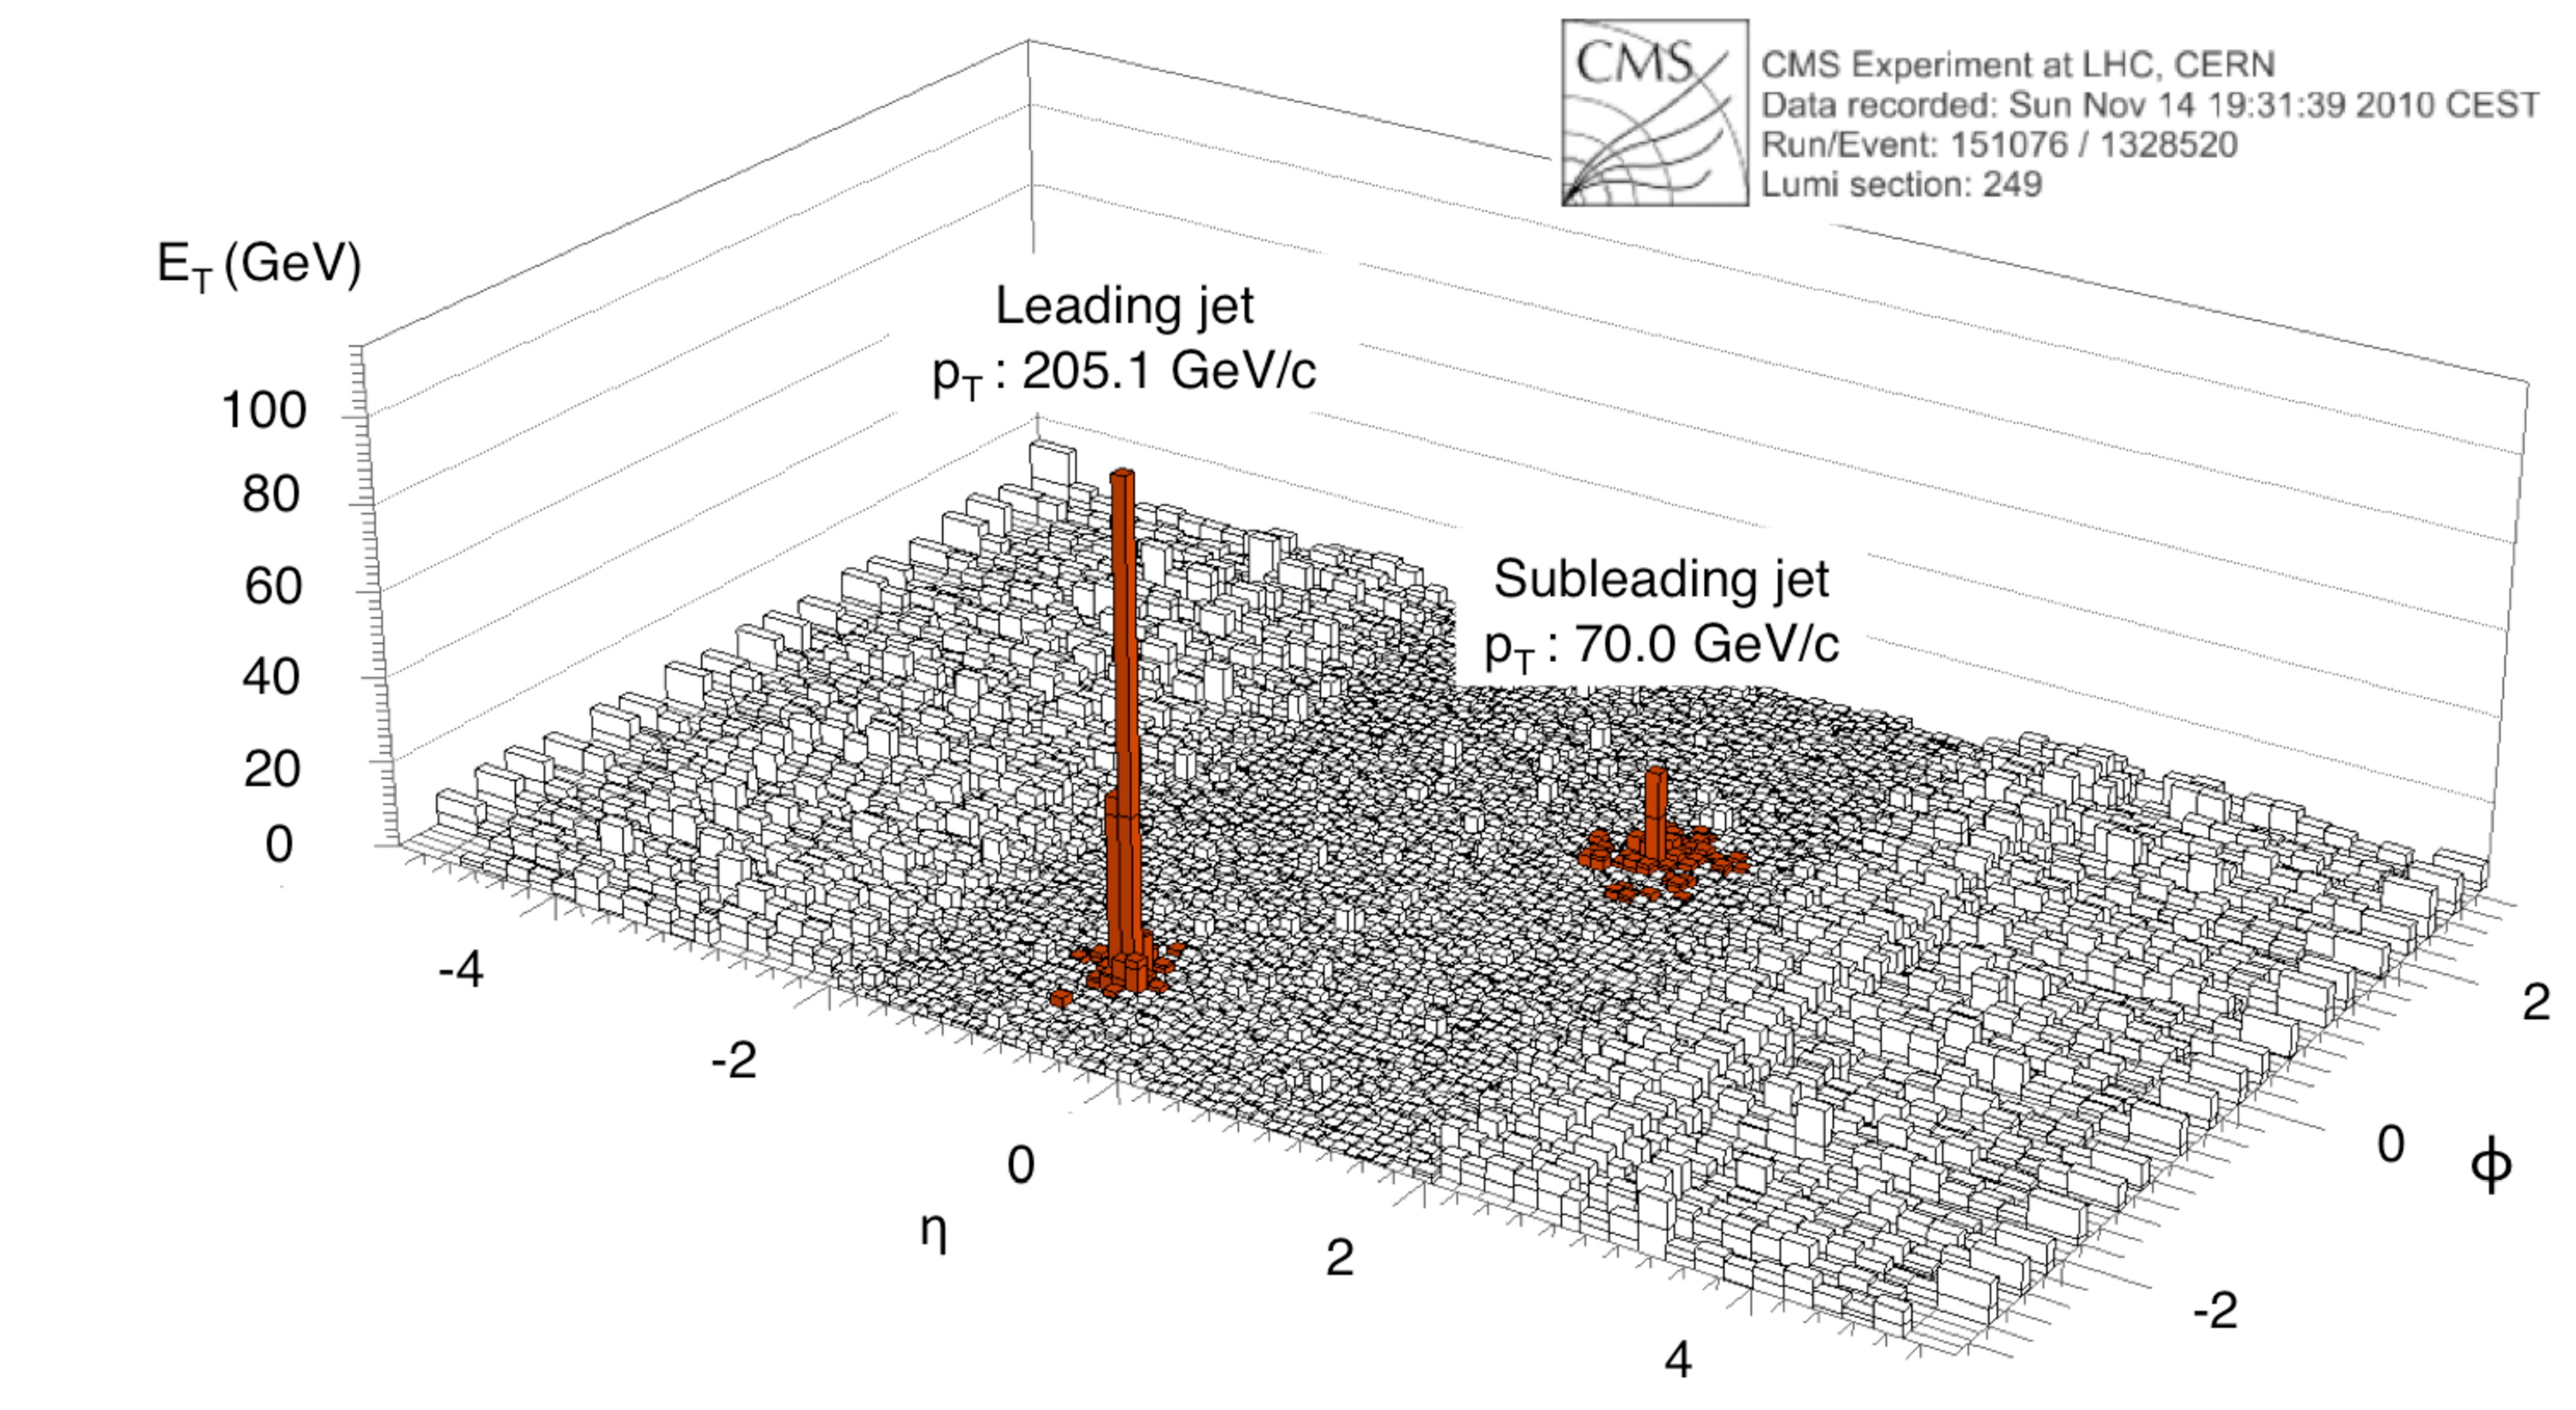
\includegraphics[width=0.6\textwidth]{01/jetquenching.pdf}
%     \end{center}
%     \item {Beyond Standard Model (BSM) physics}
%     \begin{center}
%         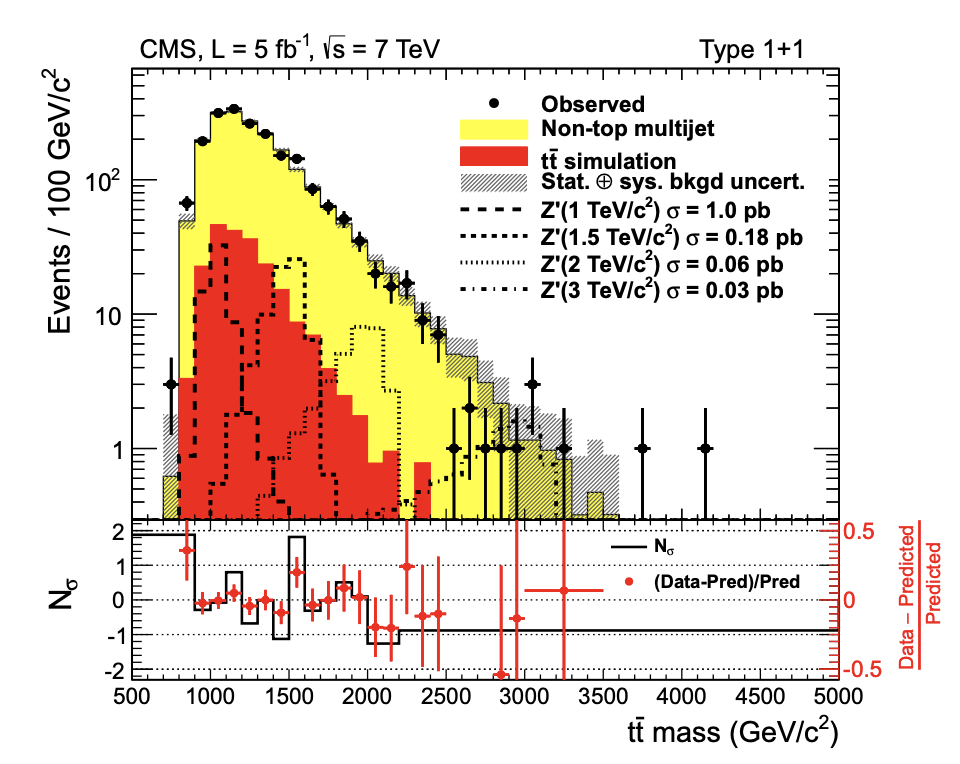
\includegraphics[width=0.7\textwidth]{01/BSM.png}
%     \end{center}
% \end{enumerate}
% \end{frame}
%
%%%%%%%%%%%%%%%%%%%%%%%%%%%%%%%%%%%%%%%%%%%%%%%%%%%%%%%%%%
%
\begin{frame}{\bf\huge Hadron collider kinematics}

{\color{red}The Large Hadron Collider (LHC)} is driving the field of jet physics:\\
\vspace{2mm}
{\color{darkred}\Large$\bullet$} The LHC is the largest and most powerful particle accelerator ever built. It delivers the {\color{darkred}most energetic collisions} (about 7 times higher than Tevatron).
\vspace{2mm}
\begin{center}
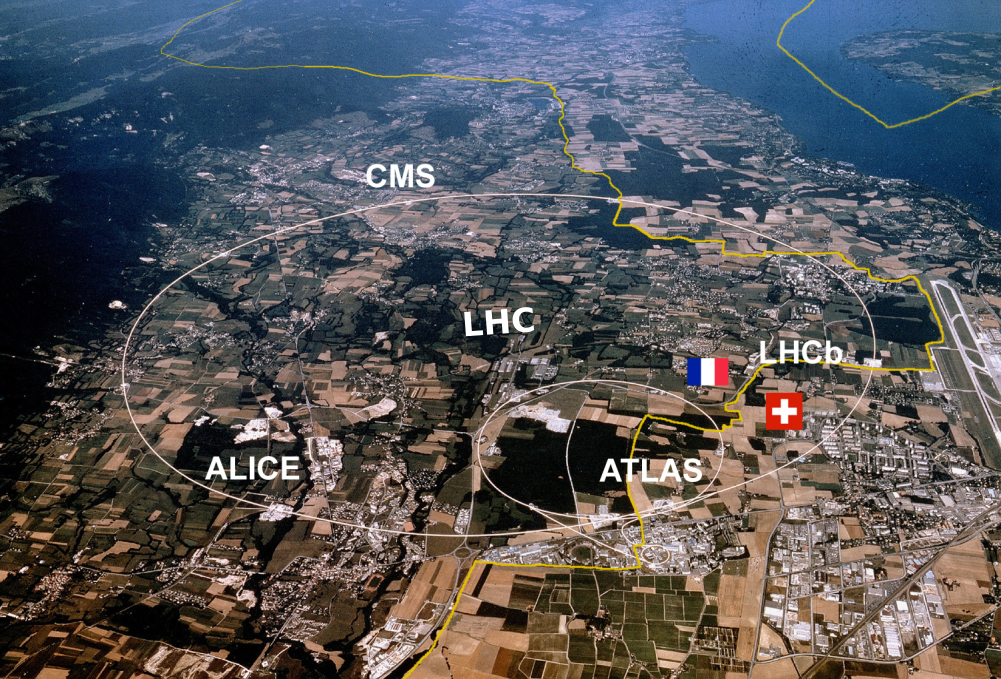
\includegraphics[width=0.6\textwidth]{LHC.png}
\end{center}
\vspace{2mm}
{\color{darkred}\Large$\bullet$} {\color{darkred} Main experiments:} ATLAS/CMS (general purpose), ALICE (heavy-ion), LHCb (b physics), all capable of studying jets.
\end{frame}
%
%%%%%%%%%%%%%%%%%%%%%%%%%%%%%%%%%%%%%%%%%%%%%%%%%%%%%%%%%%
%
\begin{frame}
\vspace{2mm}

{\color{darkred}\Large$\bullet$} {\color{darkred}The HL-LHC} (with $L\approx 5\times 10^{34}$ cm$^{-2}$ s$^{-1}$): number of collisions will be increase by about a factor of 10: to reveal more refined details of jets
\begin{center}
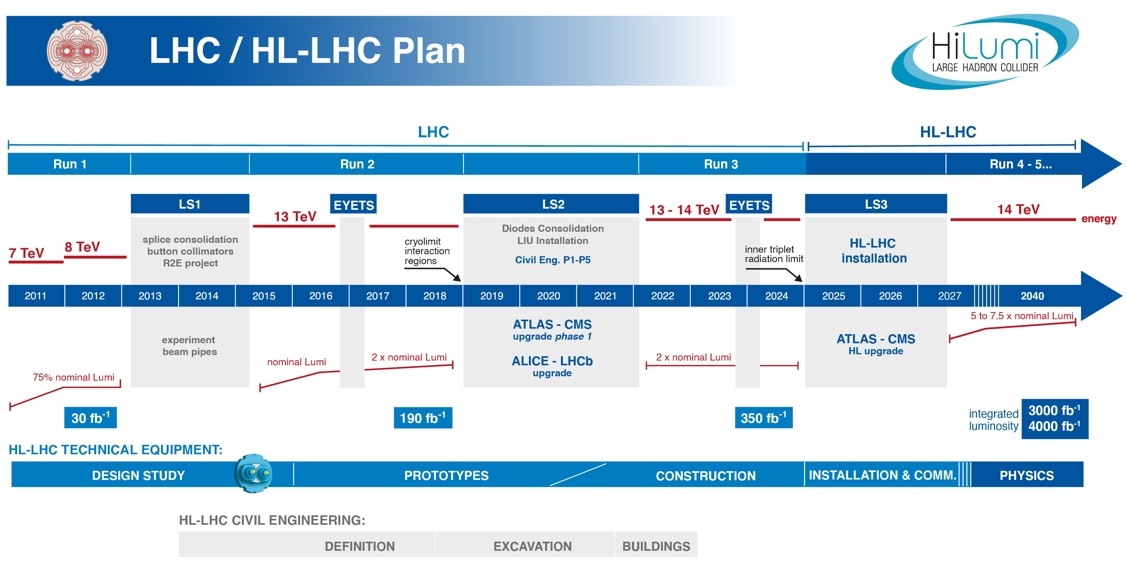
\includegraphics[width=\textwidth]{HL-LHC.png}
\end{center}
{\color{darkred}\Large$\bullet$} {\color{darkred} The total cross section} $\sigma_{tot}$ for proton-proton (pp) collisions at the LHC energies is of the order of 100 mb. About 75\% of the total events are inelastic:
\begin{align}
    \sigma_{tot}=(110.6\pm3.4)~\text{mb}\qquad \sigma_{inel}=(79.5\pm1.8)~\text{mb}\qquad \text{at $\sqrt{s}$=13 TeV}\notag
\end{align}
\begin{center}
    {\tiny\color{teablue}
    {\scshape TOTEM} collaboration,
    %\emph{{First measurement of elastic, inelastic and total cross-section at $\sqrt{s}=13$ TeV by TOTEM and overview of cross-section data at LHC energies}},
  \href{https://doi.org/10.1140/epjc/s10052-019-6567-0}{\emph{Eur. Phys. J. C}
  {\bfseries 79} (2019) 103}
  [\href{https://arxiv.org/abs/1712.06153}{{\ttfamily 1712.06153}}].}
\end{center}
\end{frame}
%
%%%%%%%%%%%%%%%%%%%%%%%%%%%%%%%%%%%%%%%%%%%%%%%%%%%%%%%%%%
%
\begin{frame}
\vspace{2mm}

{\color{darkred}\Large$\bullet$} Jets are most abundant hard "particles" produced at hadron colliders:
\begin{center}
\begin{overpic}[width=\textwidth]{01/jetsig.png}
 \put (40,50) {$L\sim 10^{34}$ cm$^{-1}$ s$^{-1}$}
\end{overpic}
\\\vspace{1mm}
 {\color{darkred}How many collisions are needed to produce one jet with $p_T> 100$ GeV?}
\end{center}
\end{frame}

%
%%%%%%%%%%%%%%%%%%%%%%%%%%%%%%%%%%%%%%%%%%%%%%%%%%%%%%%%%%
%
\begin{frame}

{\color{darkred}\Large$\bullet$} {\bf Layers of a general-purpose detector:}
% \begin{columns}
% \column{0.5\textwidth}
\begin{center}
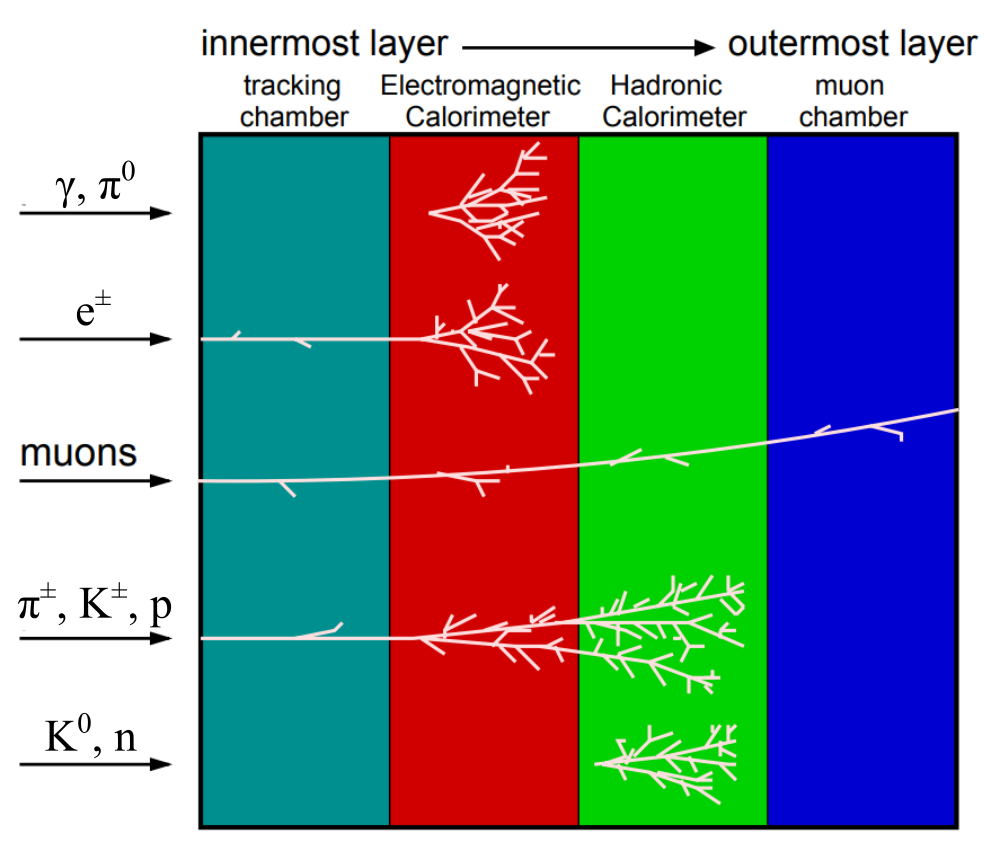
\includegraphics[width=0.6\textwidth]{01/detection.png}
\end{center}
\begin{enumerate}
    \item {\bf The tracking detectors:} tracks of charged particles
    \item {\bf The electromagnetic calorimeter:} predominantly energies of $e^\pm$ \& $\gamma$
    \item {\bf The hadron calorimeter:} energies of hadrons
    \item {\bf The muon spectrometer:} tracks of muons
\end{enumerate}
%\end{columns}
\end{frame}
%
%%%%%%%%%%%%%%%%%%%%%%%%%%%%%%%%%%%%%%%%%%%%%%%%%%%%%%%%%%
%
\begin{frame}\vspace{2mm}

{\color{darkred}\Large$\bullet$} ATLAS/CMS calorimeters have {\color{darkred}finer segmentation}:

\begin{center}
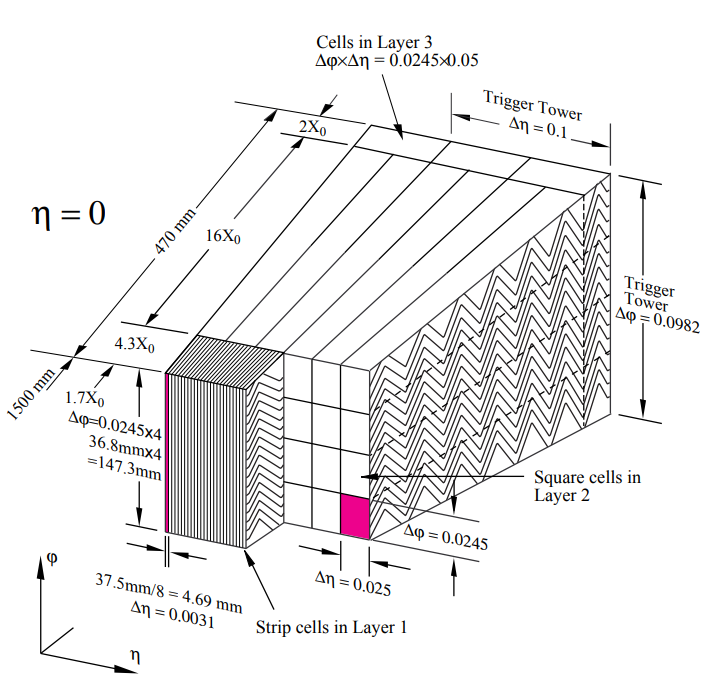
\includegraphics[width=0.6\textwidth]{01/granularity.png}
\end{center}

In the central region of the detector, the granularity for
\begin{enumerate}
    \item[\diamondsuit] {\color{red} The electromagnetic calorimeter:} $\approx(0.025\times 0.025)$ in the ($\eta$ - $\phi$) plane
    \item[\diamondsuit] {\color{red} The hadron calorimeter:} $\approx(0.1\times 0.1)$ in the ($\eta$ - $\phi$) plane
\end{enumerate}
%\end{columns}
\end{frame}

%
%%%%%%%%%%%%%%%%%%%%%%%%%%%%%%%%%%%%%%%%%%%%%%%%%%%%%%%%%%
%
\begin{frame}
\vspace{2mm}
{\color{darkred}\Large$\bullet$} {\bf The coordinate system for hadron colliders:}\\
\begin{center}
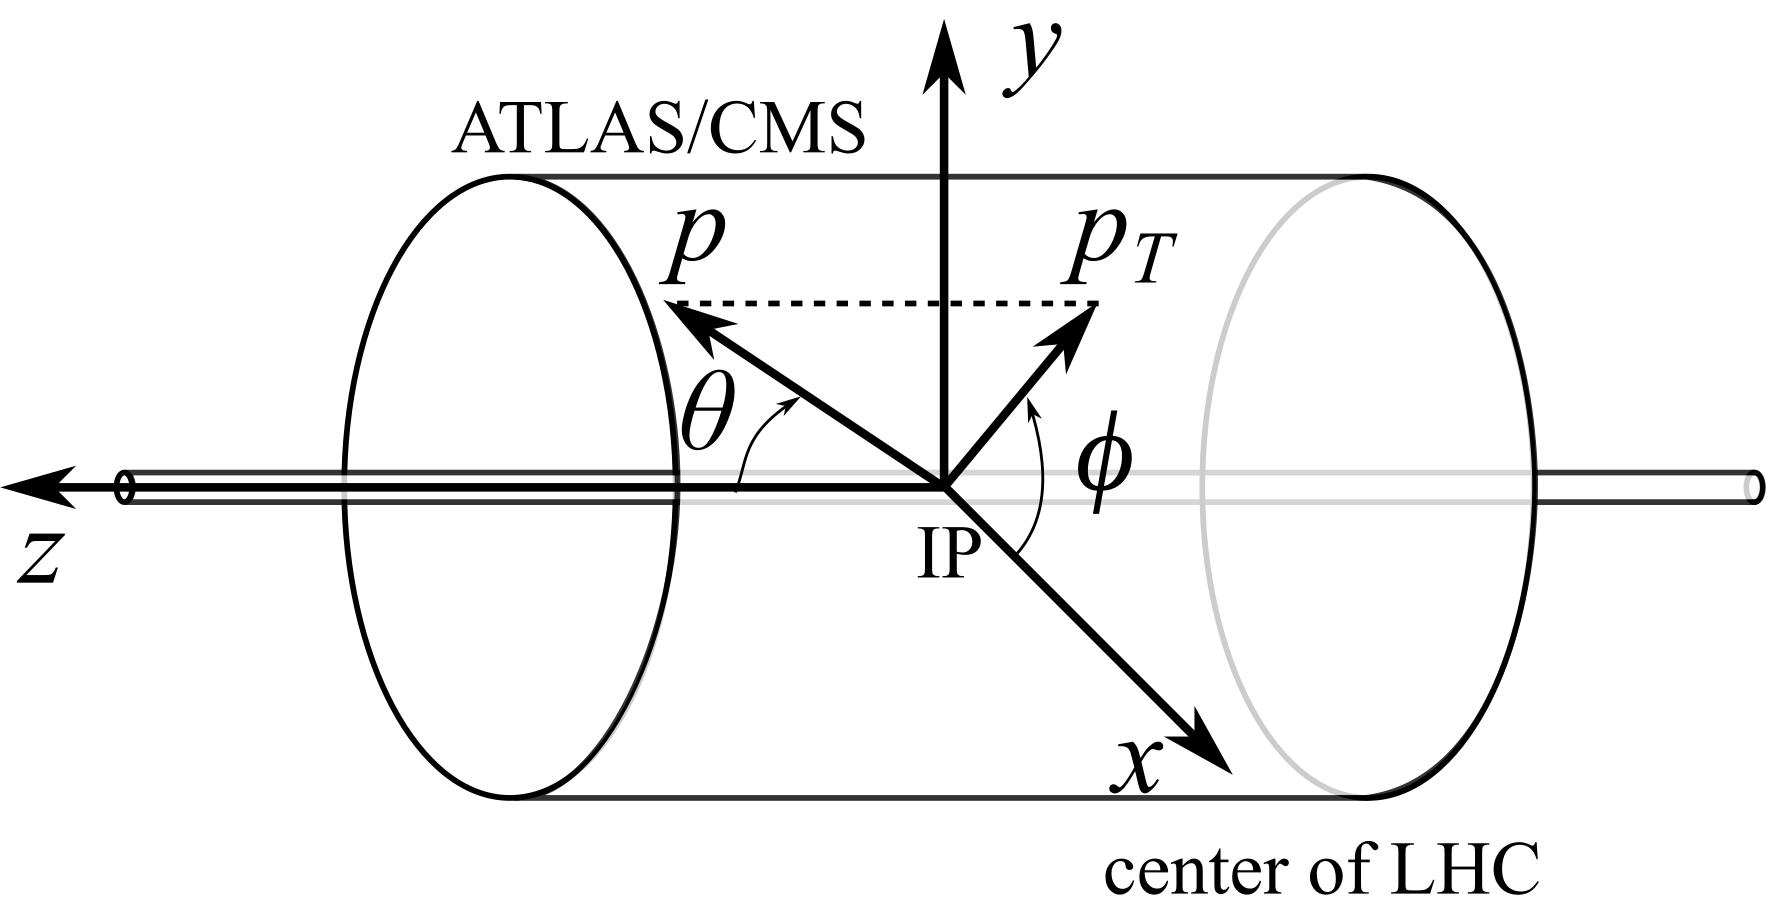
\includegraphics[width=0.6\textwidth]{coordinate.png}\\
\vspace{1mm}
$\phi$: azimuthal angle\qquad $\theta$: polar angle
\end{center}
\vspace{1mm}
{\color{darkred}\Large$\bullet$} For a particle with $p^\mu = (E, p_x, p_y, p_z)$ with $E=\sqrt{|\vec{p}|^2 + m^2}$
\vspace{2mm}
\begin{itemize}
    \item[\diamondsuit] The transverse momentum $p_T=\sqrt{p_x^2+p_y^2}$
    \vspace{2mm}
    \item[\diamondsuit] The transverse energy $E_T = E \sin\theta$
    \vspace{2mm}
    \item[\diamondsuit] The transverse mass $m_T \equiv \sqrt{p_T^2 + m^2}$
\end{itemize}
\end{frame}
%
%%%%%%%%%%%%%%%%%%%%%%%%%%%%%%%%%%%%%%%%%%%%%%%%%%%%%%%%%%
%
\begin{frame}
\vspace{2mm}
{\color{darkred}\Large$\bullet$} {\bf Rapidity:} 
$
y=\frac{1}{2}\log\left(\frac{E+p_z}{E-p_z}\right)\notag
$
In terms of $y$, $\phi$, $m_T$ and $p_T$
\begin{align}
 p^\mu=(m_T\cosh y, p_T\cos\phi, p_T\sin\phi, m_T\sinh y)\notag 
\end{align}\\
\vspace{1mm}
Accordingly $\int\frac{d^4p}{(2\pi)^4} (2\pi)\delta(p^2-m^2)\theta(p^0)=\int dy\frac{d^2p_T}{2(2\pi)^3}$.
\vspace{4mm}

{\color{darkred}\Large$\bullet$} {\bf Distance} between two particles in the $(y, \phi)$ plane:

\begin{align}
    \Delta R_{12}=\sqrt{(y_1-y_2)^2 + (\phi_1-\phi_2)^2}\equiv \sqrt{\Delta y^2_{12}+\Delta \phi^2_{12}},\notag
\end{align}
\vspace{2mm}

which is longitudinally boost-invariant. ({\color{darkred} HW1: prove this!}) Recall that Lorentz boost along the $z$-axis
\begin{align}
    \Lambda(\xi)=\left(\begin{array}{c c c c}
         \cosh\xi & 0 & 0 & \sinh\xi\\
         9 & 1 & 0 & 0 \\
         0 & 0 & 1 & 0\\
         \sinh\xi & 0 & 0 & \cosh\xi
    \end{array}\right)\notag
\end{align}
\end{frame}
%
%%%%%%%%%%%%%%%%%%%%%%%%%%%%%%%%%%%%%%%%%%%%%%%%%%%%%%%%%%
%
\begin{frame}



{\color{darkred}\Large$\bullet$} {\bf Pseudorapidity:}
$
\eta=\frac{1}{2}\log\left(\frac{|\vec{p}|+p_z}{|\vec{p}|-p_z}\right)=-\log\left(\tan\frac{\theta}{2}\right)
$\\\vspace{2mm}
Equivalently, one has
$
\cos\theta=\frac{e^{2\eta}-1}{e^{2\eta} + 1}$

\begin{center}
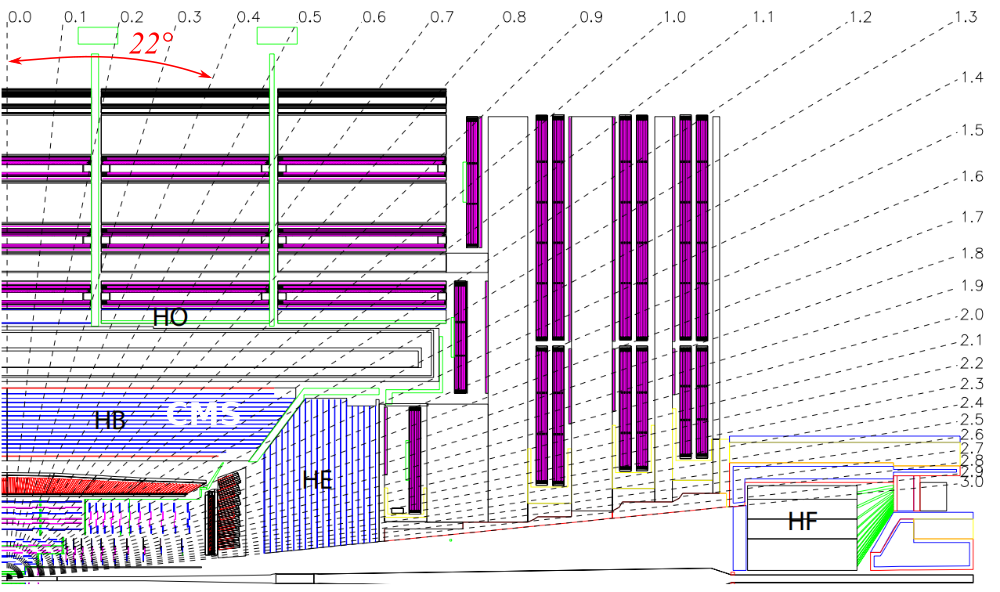
\includegraphics[width=0.9\textwidth]{eta.png}\\
\vspace{2mm}
\begin{tabular}{ |c| c c c c c c c c c c c|}
\hline\hline
 $\eta$ & 0 & 0.1 & 0.2 & 0.3 & 0.4 & 0.5 & 0.6 & 1 & 2 & 3 & 4 \\ 
 \hline
 $\theta$ & 90$^\circ$ & 84$^\circ$ & 79$^\circ$ & 73$^\circ$ & 68$^\circ$ &
       62$^\circ$ & 58$^\circ$ & 40$^\circ$ & 15$^\circ$ &  5.7$^\circ$ &
        2.1$^\circ$\\
 \hline
\end{tabular}
\end{center}
\end{frame}
%
%%%%%%%%%%%%%%%%%%%%%%%%%%%%%%%%%%%%%%%%%%%%%%%%%%%%%%%%%%
%
\begin{frame}\vspace{4mm}

{\color{darkred}\Large$\bullet$} A fun fact about $R=0.4$ jets: {\color{darkred}$2R\approx 44^\circ$ in $\theta$ and 46^\circ$ in $\phi$} in central region\vspace{2mm}

\begin{center}
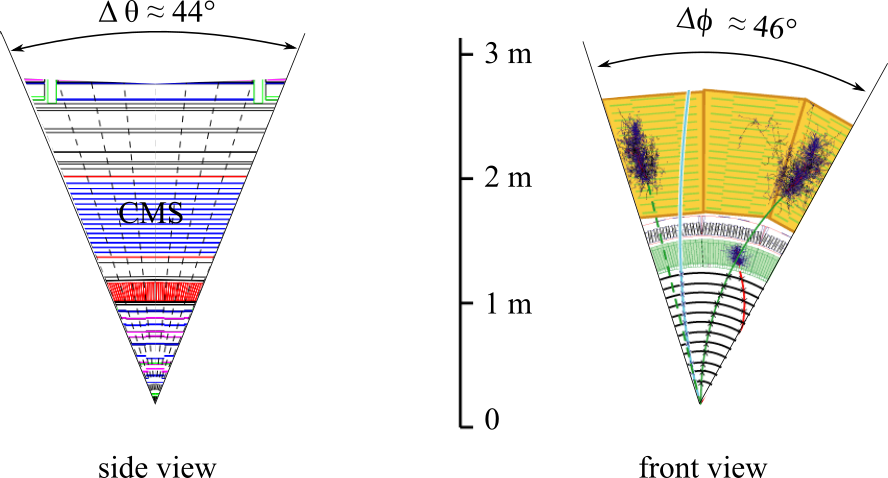
\includegraphics[width=\textwidth]{01/R4jets.png}\\
\vspace{4mm}
Jets will be measured by a cone $\approx 3$ m high with opening angle $\approx 45^\circ$.
\end{center}
\end{frame}

%
%%%%%%%%%%%%%%%%%%%%%%%%%%%%%%%%%%%%%%%%%%%%%%%%%%%%%%%%%%
%
\begin{frame}

{\color{darkred}\Large$\bullet$} It is common to present {\bf jet events} in the $(\eta, \phi)$ plane:
\begin{center}
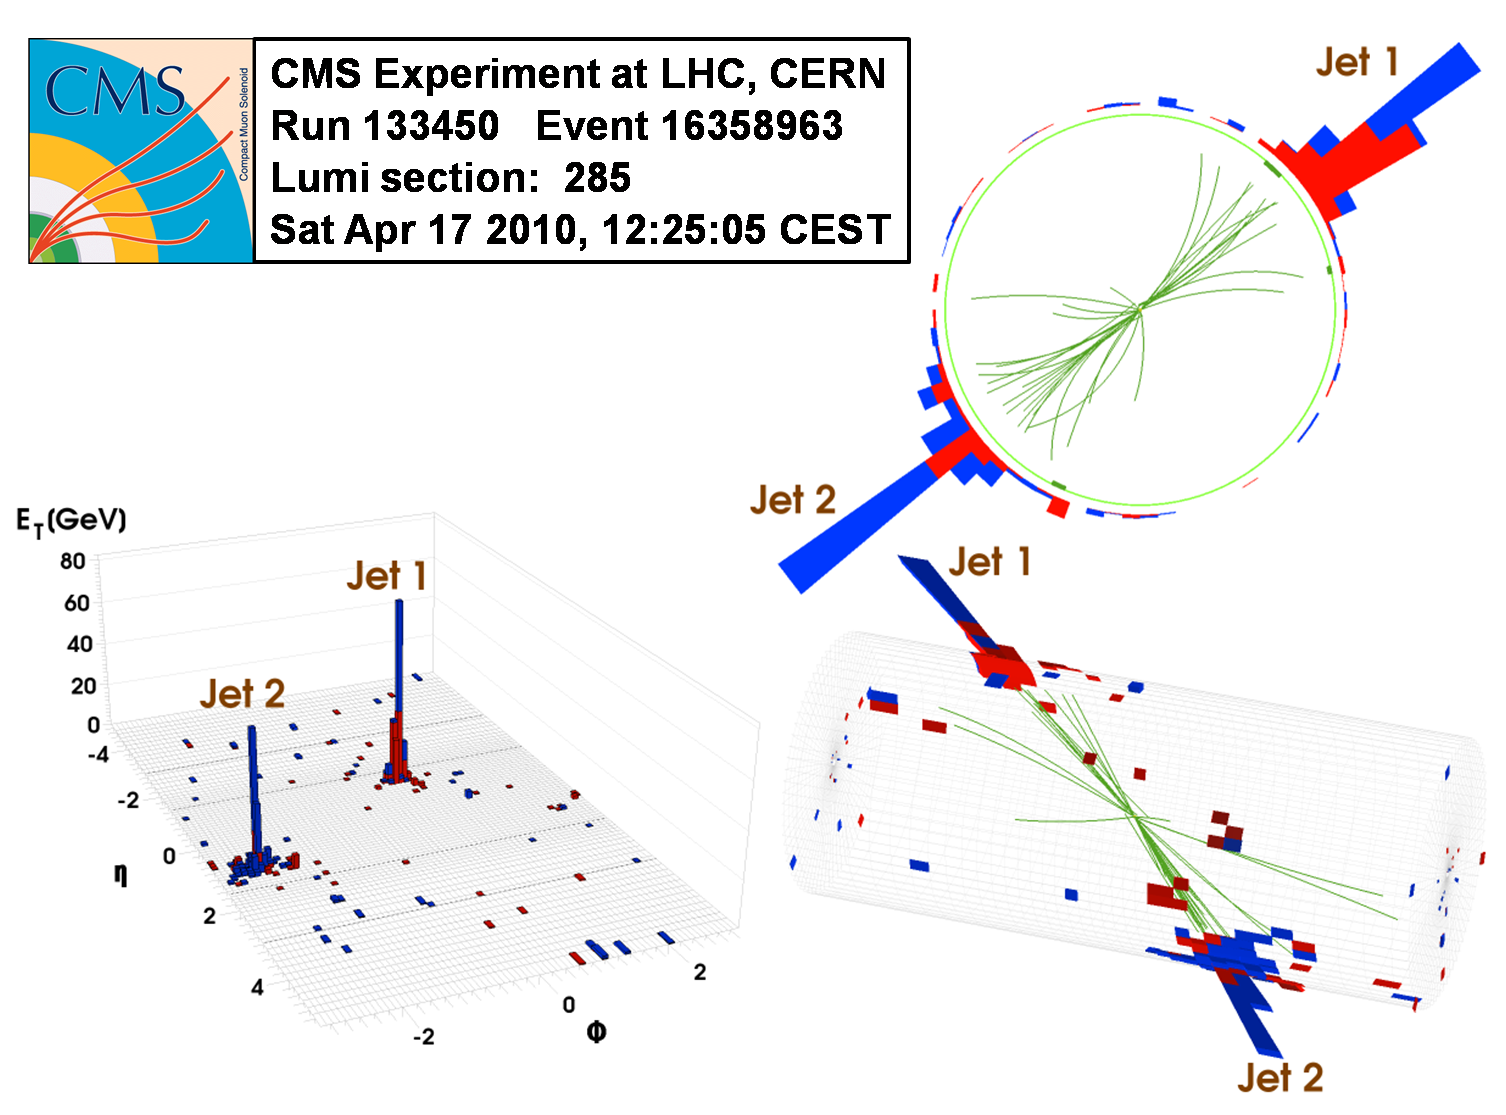
\includegraphics[width=0.8\textwidth]{lego.png}\\
\vspace{1mm}
{\small({\color{red}red for ECAL}, {\color{blue}blue for HCAL})}\\
\vspace{1mm}
{\tiny
\href{https://twiki.cern.ch/twiki/bin/view/CMSPublic/PhysicsResultsJME}{https://twiki.cern.ch/twiki/bin/view/CMSPublic/PhysicsResultsJME}
}
\end{center}
\end{frame}
%
%%%%%%%%%%%%%%%%%%%%%%%%%%%%%%%%%%%%%%%%%%%%%%%%%%%%%%%%%%
%
\begin{frame}{\bf\huge \centering{What are jets?}}
\vspace{2mm}
{\color{darkred}\Large$\bullet$} {\bf Jets} are collimated sprays of hadrons.\\
\vspace{2mm}
{\color{darkred}\Large$\bullet$} Jets emerge from {\bf Quantum Chromodynamics (QCD)}:\\
\vspace{1mm}
\begin{center}
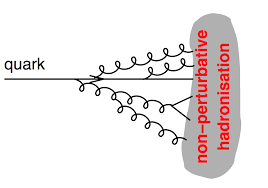
\includegraphics[width=0.5\textwidth]{jetform.png}\\
\end{center}
\begin{enumerate}
    \item {\color{darkred}Usually}, a jet is initiated by a high-$p_T$ parton created in some hard process.
    \item It, then, radiates and produces a collimated parton shower.
    \item Finally, it hadronizes, turning into hadrons to be observed in the detector.
\end{enumerate}
We call this kind of jets {\color{darkred}QCD jets}.
\end{frame}
%
%%%%%%%%%%%%%%%%%%%%%%%%%%%%%%%%%%%%%%%%%%%%%%%%%%%%%%%%%%
%
\begin{frame}
\vspace{2mm}

{\color{darkred}\Large$\bullet$} Messiness  in pp collisions:\\
\vspace{2mm}
\begin{center}
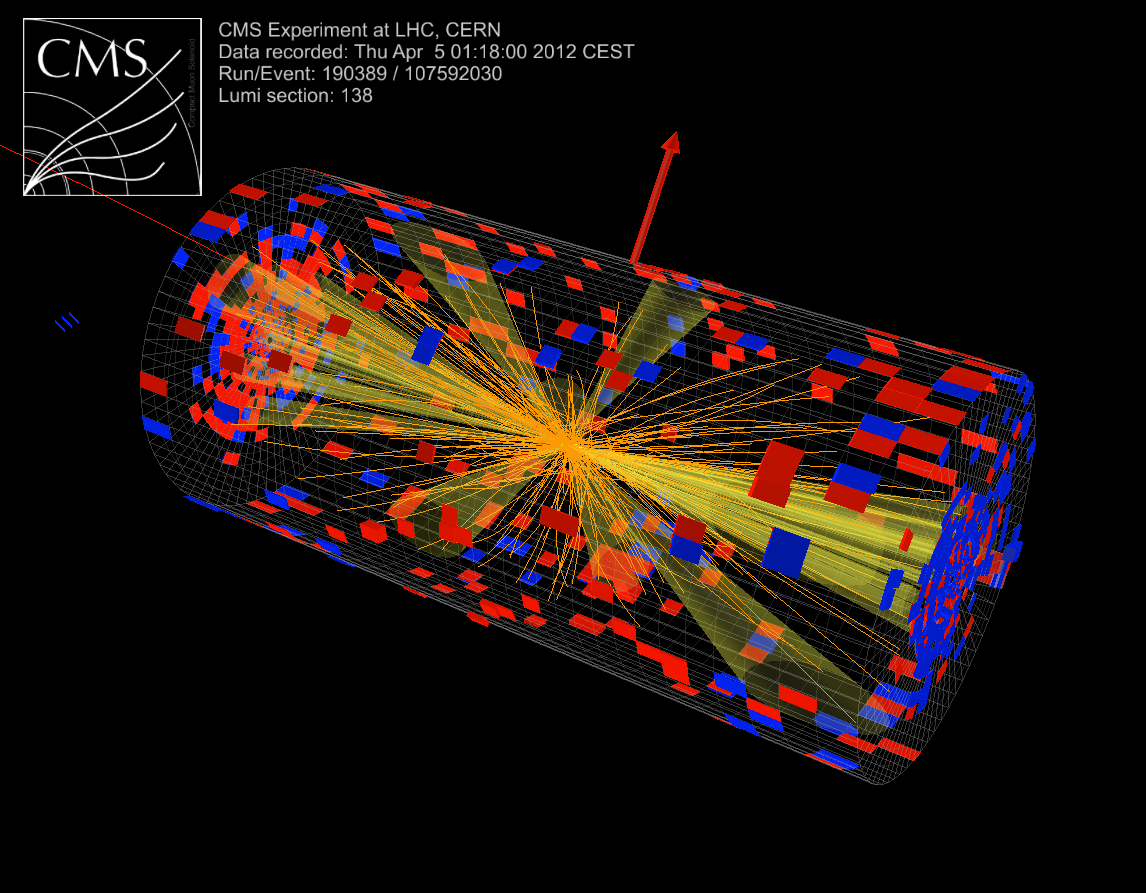
\includegraphics[width=0.7\textwidth]{pp.png}\\
\vspace{2mm}
O(500) particles produced, most of which carry small $p_T$ and are regarded as {\color{darkred}underlying event (UE)}.
\end{center}
% {\color{darkred}\Large$\bullet$} In experiments:\\
% \begin{align}
%     \begin{minipage}[c]{0.2\textwidth}
%     \begin{center}
%  Jets
%     \end{center}
% \end{minipage}
% =
% \begin{minipage}[c]{0.2\textwidth}
%     \begin{center}
%     clusters\\
%     of\\
%     desired\\
%     hadrons
%     \end{center}
% \end{minipage}
% +
% \begin{minipage}[c]{0.2\textwidth}
%     \begin{center}
%     contamination
%     \end{center}
% \end{minipage}\notag
% \end{align}
\end{frame}
%
%%%%%%%%%%%%%%%%%%%%%%%%%%%%%%%%%%%%%%%%%%%%%%%%%%%%%%%%%%
%
\begin{frame}
\vspace{2mm}

\begin{columns}
\begin{column}{0.5\textwidth}
\begin{center}
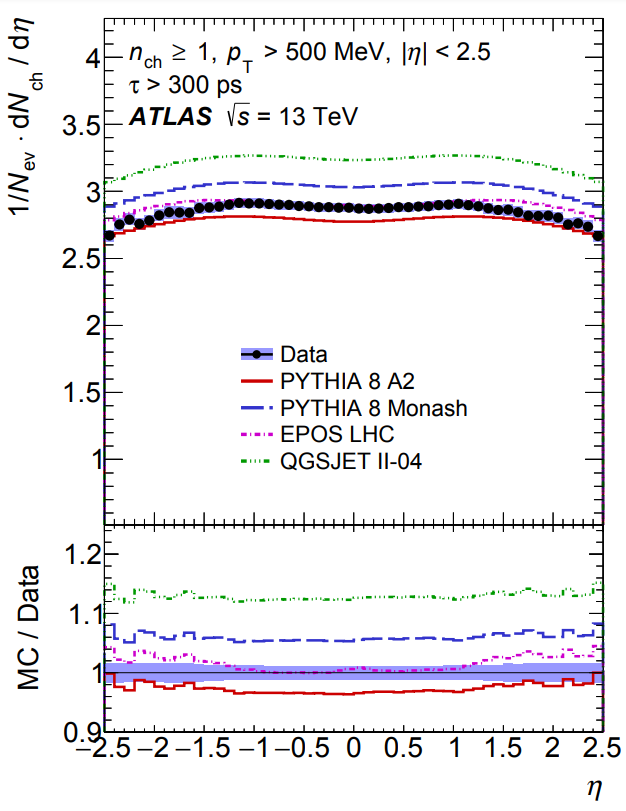
\includegraphics[width=\textwidth]{01/multiplicity.png}\\
    {\tiny \color{teablue}{\scshape ATLAS} collaboration, %\emph{{Charged-particle distributions in $\sqrt{s}$ = 13 TeV pp interactions measured with the ATLAS detector at the  LHC}},
    \href{https://doi.org/10.1016/j.physletb.2016.04.050}{\emph{Phys.
  Lett. B} {\bfseries 758} (2016) 67}
  [\href{https://arxiv.org/abs/1602.01633}{{\ttfamily 1602.01633}}].
}
\end{center}
\end{column}

\begin{column}{0.5\textwidth}
{\color{darkred}\Large$\bullet$} {\bf Longitudinal boost-invariance:}\\\vspace{1mm}
In the central rapidity region, the particle production is relatively constant.\\
\vspace{2mm}
At LHC energies, there is O(1) particle (pion) for each unit area on the $(\eta, \phi)$ plane.
\\
\vspace{2mm}
{\color{darkred}\Large$\bullet$} {\bf Pileup:} the average number of collisions
produced per bunch crossing:
\begin{center}
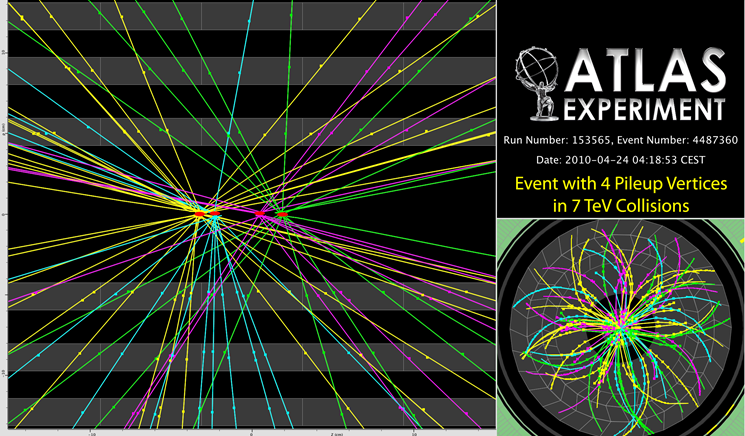
\includegraphics[width=\textwidth]{01/pileup.png}
\end{center}
\end{column}
\end{columns}
 \end{frame}
 
\begin{frame}
\vspace{2mm}

{\color{darkred}\Large$\bullet$} An estimate of pileup:\\\vspace{2mm}

The peak luminosity of the LHC is $L=2\times10^{34} cm^{-2} s^{-1}$ and 
     and bunch spacing  25 ns $\Rightarrow$ pileup = 40.\\\vspace{2mm}
     
{\color{darkred}\Large$\bullet$} Luminosity measurement at ATLAS:
\begin{center}
    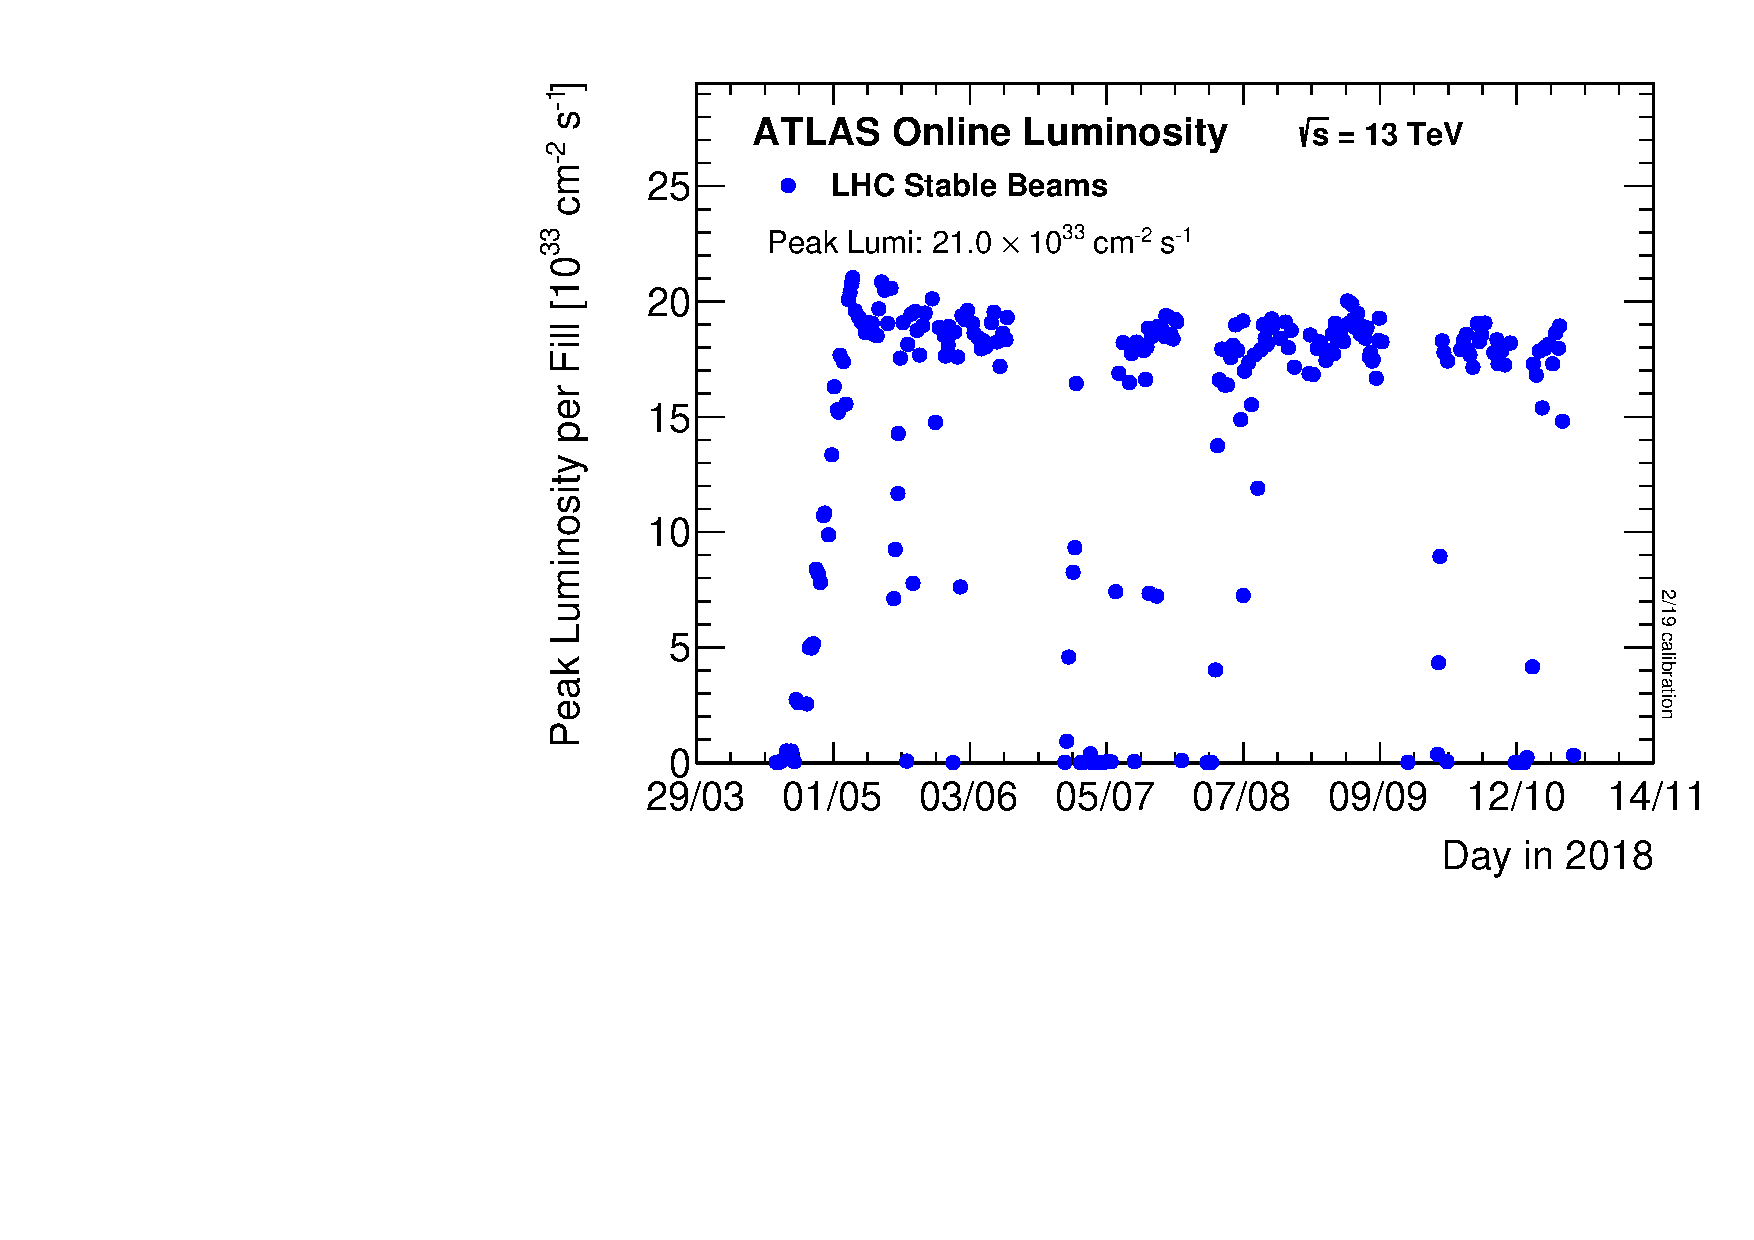
\includegraphics[width=0.45\textwidth]{01/peakLumi.pdf}
    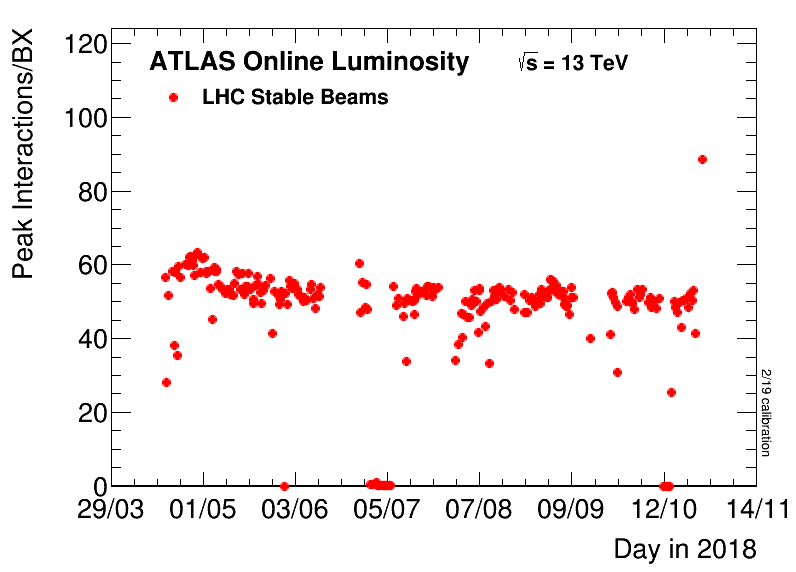
\includegraphics[width=0.45\textwidth]{01/pileupATLAS.png}\\\vspace{1mm}
    {\tiny\href{https://twiki.cern.ch/twiki/bin/view/AtlasPublic/LuminosityPublicResultsRun2}{https://twiki.cern.ch/twiki/bin/view/AtlasPublic/LuminosityPublicResultsRun2}}
\end{center}
\vspace{2mm}

{\color{darkred}\Large$\bullet$} Pileup presents a challenge to the reconstruction of jets. We need one of the collision to be hard to produce jets but it overlays in the detector with all the other mostly soft collisions in the same bunch crossing.

\end{frame}
%
%%%%%%%%%%%%%%%%%%%%%%%%%%%%%%%%%%%%%%%%%%%%%%%%%%%%%%%%%%
%
\begin{frame}\vspace{2mm}

{\color{darkred}\Large$\bullet$} Jets are reconstructed from {\bf energy deposits} in calorimeters:\\
\vspace{1mm}
\begin{itemize}
    \item[\diamondsuit] {\bf CMS:} clusters of {\it particle flow} objects, as combining information from trackers and calorimeters
    \item[\diamondsuit] {\bf ATLAS:} {\it topological clusters} mainly based on calorimeters for runs 1 \& 2; {\it particle flow} objects for future runs.
\end{itemize}
\vspace{1mm}

{\color{darkred}\Large$\bullet$} At $\sqrt{s}=7$ TeV, charged
hadrons were found to carry on average 65\% of the jet energy, photons 25\% and neutral hadrons
10\%. 
\begin{center}
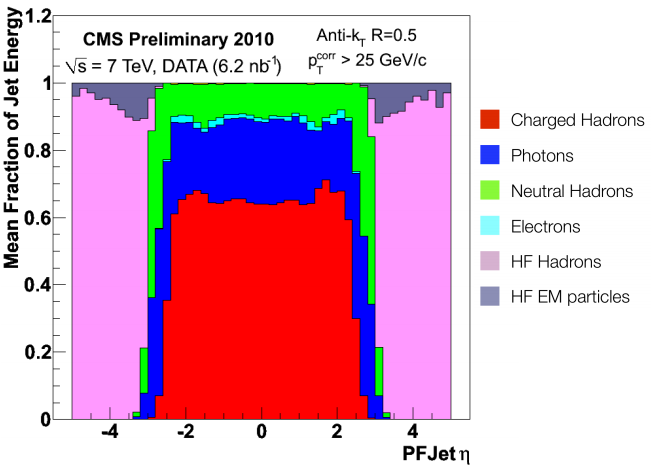
\includegraphics[width=0.5\textwidth]{01/jetchem.png}\\
{\tiny\color{teablue}
{\scshape CMS} collaboration, %\emph{{Commissioning of the Particle-Flow reconstruction in Minimum-Bias and Jet Events from pp Collisions at 7 TeV}}
\href{https://inspirehep.net/files/01f35fa9e56c5e0c30f1b9b4c0560656}{CMS-PAS-PFT-10-002}.}
\end{center}

{\color{darkred}\Large$\bullet$} At LHC energies, a jet typically is a group of (10-30) hadrons including pions: $\approx$80\%, kions: $\approx$15\% and anything else: $\approx$5\%. 
\end{frame}
%
%
%%%%%%%%%%%%%%%%%%%%%%%%%%%%%%%%%%%%%%%%%%%%%%%%%%%%%%%%%%
%
\begin{frame}{\bf\huge \centering{Jet definition}}
\vspace{2mm}
{\color{darkred}\Large$\bullet$} Jets need to be {\bf defined} because they are arbitrary. A jet definition includes:\\
%\vspace{2mm}
\begin{enumerate}
    \item[\diamondsuit] {Jet algorithm:} {\it a set of rules to group "particles" into jets}
    \item[\diamondsuit] {Recombination scheme:} {\it how to assign a momentum to the resulting jet}
\end{enumerate}
The first jet finding dates back to:
    {\tiny\color{teablue}G.F.~Sterman and S.~Weinberg, %\emph{{Jets from Quantum Chromodynamics}},
  \href{https://doi.org/10.1103/PhysRevLett.39.1436}{\emph{Phys. Rev. Lett.}
  {\bfseries 39} (1977) 1436}.}\\
\vspace{2mm}
{\color{darkred}\Large$\bullet$} Most jet algorithms can be classified into two classes:\\
%\vspace{2mm}
\begin{enumerate}
    \item[\diamondsuit] {Cone algorithms:} \\{\it Group particles within specific conical angular regions into jets.}
    \item[\diamondsuit] {\color{darkred} Sequential recombination algorithms:} the main kind in use at the LHC\\{\it First, define some
distance measure between particles. Then, repeatedly replace the pair of particles that are closest with a particle constructed by recombining these two particles until some stopping criterion is reached.}
\end{enumerate}
\vspace{2mm}
{\color{darkred}\Large$\bullet$} Criteria for a good jet definition:\\
\begin{align}
    \begin{minipage}[c]{0.2\textwidth}
    \begin{center}
  clusters\\
  of\\
  partons
    \end{center}
\end{minipage}
\approx
\begin{minipage}[c]{0.2\textwidth}
    \begin{center}
  clusters\\
  of\\
  hadrons
    \end{center}
\end{minipage}
\approx
\begin{minipage}[c]{0.2\textwidth}
    \begin{center}
  clusters\\
  of\\
  measurements
    \end{center}
\end{minipage}\notag
\end{align}
\begin{center}
    {\color{darkred} Topic for lecture 3.}
\end{center}
\end{frame}
%
%%%%%%%%%%%%%%%%%%%%%%%%%%%%%%%%%%%%%%%%%%%%%%%%%%%%%%%%%%
%
\begin{frame}{\bf\huge \centering{Jets of different origin}}
\vspace{2mm}
{\color{darkred}\Large$\bullet$} Traditional {\color{red}QCD jets}: one-prong structure\\
\vspace{1mm}
\begin{center}
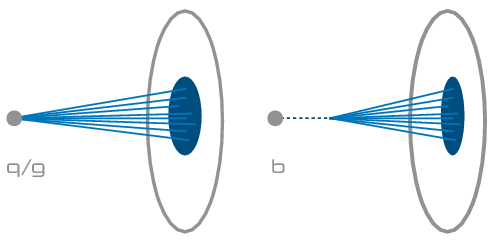
\includegraphics[width=0.5\textwidth]{01/qcdjets.png}
\end{center}
b jets can be discriminated from jets produced by the hadronization of light quarks based on characteristic properties of B hadrons, such as the long lifetime.\\
\vspace{2mm}
QCD jets are massive. And we will discussion {\color{darkred}jet mass in Lecture 4}.
\end{frame}
%
%%%%%%%%%%%%%%%%%%%%%%%%%%%%%%%%%%%%%%%%%%%%%%%%%%%%%%%%%%
%
\begin{frame}
\vspace{2mm}

{\color{darkred}\Large$\bullet$} Highly boosted $W^\pm, Z^0, H^0\to q\bar{q}$: {\color{red}two-pronged fat jets}\\
\vspace{1mm}
\begin{center}
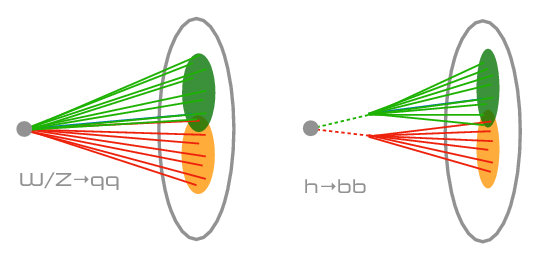
\includegraphics[width=0.5\textwidth]{01/bosonjets.png}
\end{center}
\vspace{2mm}
{\color{darkred}\Large$\bullet$} Highly boosted top quarks: {\color{red}three-pronged fat jets}\\
\vspace{1mm}
\begin{center}
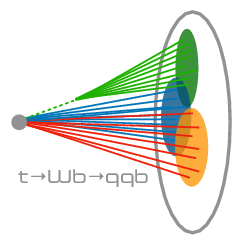
\includegraphics[width=0.3\textwidth]{01/tjets.png}
\end{center}


\end{frame}
%
%%%%%%%%%%%%%%%%%%%%%%%%%%%%%%%%%%%%%%%%%%%%%%%%%%%%%%%%%%
%
\begin{frame}
\vspace{2mm}

{\color{darkred}\Large$\bullet$} Decay of heavy BSM particles: $\Rightarrow$ fat jets\\
\begin{center}
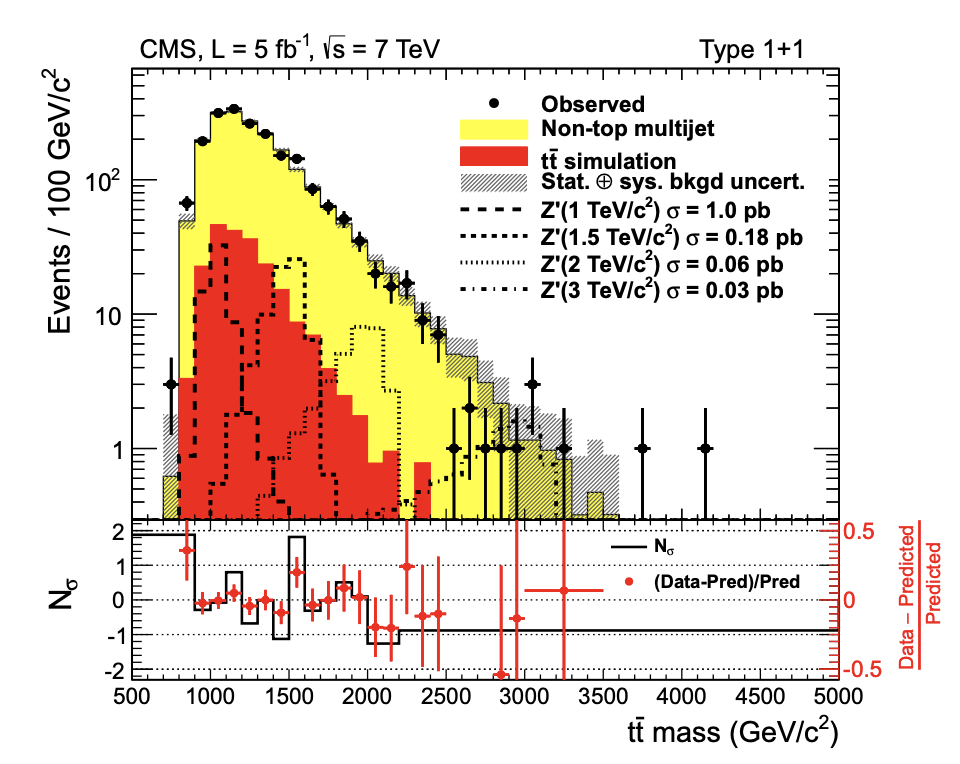
\includegraphics[width=0.7\textwidth]{01/BSM.png}
\end{center}
\vspace{1mm}
{\color{darkred}\Large$\bullet$} QCD jets are usually taken as (part of ) {\bf QCD backgrounds}. One needs to find ways to separate interested processes ({\bf signal}) involving fat jets from the QCD backgrounds.\\
\vspace{1mm}
{\color{darkred}\Large$\bullet$} {\bf\color{darkred} Jet substructure methods} tell apart various fat jets from QCD jets by investigating their internal structure. They usually include two steps:\\
\vspace{1mm}
\begin{enumerate}
    \item Clean up/groom the jet by removing soft radiation
    \vspace{1mm}
    \item Use the remaining hard constituents of the jet to separate signal and background jets. Specific observables are designed to discern the one-prong, two-prong, three-prong or novel BSM structures in the previous example. 
\end{enumerate}
\begin{center}
    {\color{darkred}Topic for Lectures 5-7}
\end{center}
\end{frame}
\end{document}